\documentclass{beamer}

\usepackage[utf8]{inputenc}
\usepackage[english]{babel}
\usepackage[T1]{fontenc}

%\usepackage{multicol}

\title{Probably Approximate Correct learning for Gene Control Networks}
\author{Arthur Carcano}
\institute{ENS}

\usetheme{Singapore}
\usecolortheme{default}

\usepackage{color}
\usepackage{subcaption}
\usepackage{adjustbox}
\usepackage{algpseudocode}

\usepackage{verbatim}

\newcommand{\transition}{\vspace{1em}\flushright \itshape}
\newcommand{\ok}{\textcolor{blue}{\checkmark}}
\newcommand{\nope}{\textcolor{red}{$\times$}}

\begin{document}
	
	\frame{
		\titlepage
	}
	
	\frame{
	\tableofcontents
}
	\section{The problem}
	\subsection{Statement}
	\begin{frame}
		\frametitle{The problem}
		\begin{itemize}
			\item We want to learn $F : \mathbb{B}^s \longrightarrow \mathbb{B}$
			\item With:
			\begin{itemize}
					\item $\mathcal{V}$ so that for every $v$ in  $\mathcal{V}$, $F(v) = 1$. (positive examples). We can get a $v$ with probability $D(v)$ by probing.
					\item An oracle able to compute $F$ for any $v$.
			\end{itemize}
		\end{itemize}
	\transition How much probing and call to the oracles do we need ?
	\end{frame}
\subsection{Two classes}
\begin{frame}
	Two classes of $F$ on which we focus:
	\begin{itemize}
		\item $k$-CNF
		\item Monotone DNF
	\end{itemize}
\end{frame}

\section{Bounds}
\subsection{k-CNF}
\begin{frame}
	\frametitle{Bounds}
	\begin{block}{L(h,S)}
			Smallest integer $i$ so that for $i$ independent Bernoulli trials with probability of success greater or equal to $h^{-1}$, the probability of having less than $S$ success is less than $h^{-1}$.
			$$L(h,S) \leq 2h\left(S+\ln(h)\right)$$
	\end{block}
	\begin{block}{k-CNF}
		\begin{itemize}
			\item $L(h,(2s)^{k+1})$ examples
			\item 0 calls to oracle
		\end{itemize}
	\end{block}
\end{frame}
\subsection{Monotonous DNF}
\begin{frame}
	\frametitle{Bounds}
	\begin{block}{L(h,S)}
		Smallest integer $i$ so that for $i$ independent Bernoulli trials with probability of success greater or equal to $h^{-1}$, the probability of having less than $S$ success is less than $h^{-1}$.
		$$L(h,S) \leq 2h\left(S+\ln(h)\right)$$
	\end{block}
	\begin{block}{Monotonous DNF}
		\begin{itemize}
			\item $L(h,d)$ examples
			\item $ds$ calls to oracle
		\end{itemize}
	\end{block}
\end{frame}
\section{Application to biology}
\begin{frame}
	\frametitle{Application to biology}
	\begin{itemize}
		\item Consider the boolean abstraction of gene expression level
		\item (De)activation function of a given gene is a boolean function
	\end{itemize}
	\transition Can we get positive examples ? Oracle ?
\end{frame}
\begin{frame}
	\frametitle{Application to biology}
	Can we get positive examples ? Oracle ? You tell me !
	\begin{itemize}
		\item Example: maybe
		\item Oracle: unlikely (nature is probabilistic)
	\end{itemize}
\end{frame}
\begin{frame}
	\frametitle{Application to biology}
	Meaning of the classes:
	\begin{description}
		\item[k-CNF] (de)activation depends on at most k compounds
		\item[monotone DNF] No inhibition
	\end{description}
\end{frame}
	\section{Algorithms}
\subsection{Algorithm for k-CNF}
\frame{
	\frametitle{Algorithm for k-CNF}
	\begin{block}{Idea}
		Compute the more constraining k-CNF true for every sample we got
	\end{block}
}
\begin{frame}
	\frametitle{Algorithm for k-CNF and monotone DNF explained on board}
	\begin{figure}
		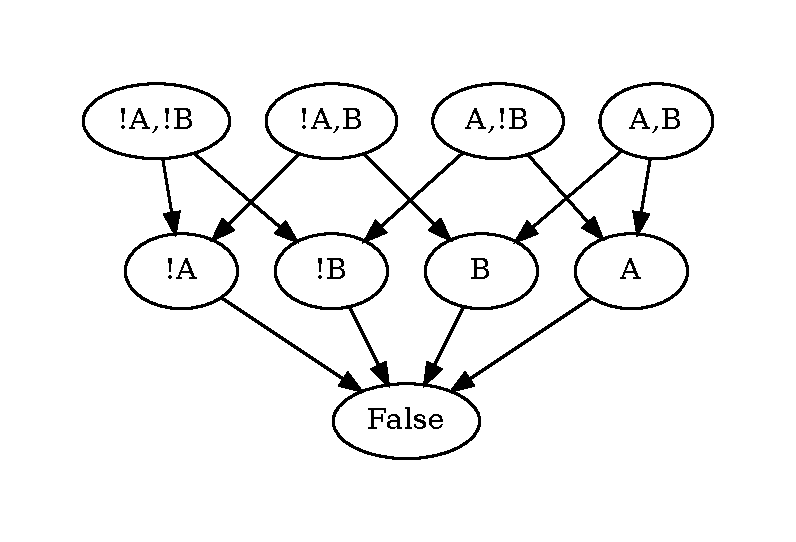
\includegraphics[height=0.9\textheight]{lattice}
	\end{figure}
\end{frame}
\section{Results}
\begin{frame}
	\frametitle{Examples}
	\begin{columns}
		\column[]{0.2\textwidth}
	\begin{figure}[htbp]
		\verbatiminput{../test.reac}
	\end{figure}%\vrule{\textheight}
	\column[]{0.7\textwidth}
	\begin{figure}[htbp]
		\verbatiminput{../Lokta.reac}
	\end{figure}
\end{columns}
\end{frame}
\begin{frame}
	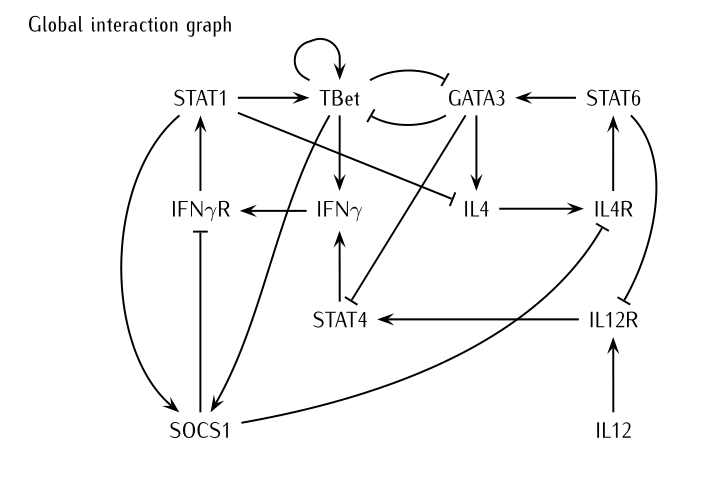
\includegraphics[height=0.8\textheight]{th_net}
\end{frame}
\begin{frame}[fragile=singleslide]
	\frametitle{Examples}
	\begin{columns}
		\column[]{0.5\textwidth}
		\begin{figure}[htbp]
			\begin{verbatim}
			{}
			-> 100*IL4 (0.01)
			-> 100*IL12 (0.01)
			TBet -> IFNg
			STAT4 -> IFNg
			GATA3 /STAT1 -> IL4
			IFNg /SOCS1 -> IFNgR
			IL4 /SOCS1 -> IL4R
			IL12 /STAT6 -> IL12R
			IFNgR -> STAT1
			IL4R -> STAT6
		\end{verbatim}
				\end{figure}
	\column[]{0.5\textwidth}
\begin{figure}[htbp]
	\begin{verbatim}
	IL12R /GATA3 -> STAT4
	STAT1 -> SOCS1
	TBet -> SOCS1
	STAT1 /GATA3 -> TBet
	TBet /GATA3 -> TBet
	STAT6 /TBet -> GATA3
	GATA3 ->
	SOCS1 ->
	\end{verbatim}
\end{figure}
	\end{columns}
\end{frame}
	\begin{frame}
		\frametitle{Examples}
			\begin{figure}[htbp]
				\verbatiminput{../test.result}
			\end{figure}%\vrule{\textheight}
	\end{frame}
	\begin{frame}
		\small
	\frametitle{Examples}
	\begin{figure}[htbp]
		\verbatiminput{../lokta.result}
	\end{figure}%\vrule{\textheight}
\end{frame}
\begin{frame}[fragile=singleslide]
	\begin{verbatim}
		IL4- : [['!SOCS1'], ['!TBet', '!GATA3']]
		TBet- : [['!GATA3']]
		STAT4+ : [['!GATA3'], ['IL12R']]
		STAT4- : [['!TBet', 'IFNg'], ['!TBet', '!GATA3']]
		GATA3+ : [['!TBet'], ['STAT6']]
		GATA3- : [['!TBet']]
		STAT1+ : [['IFNgR'], ['!TBet', '!GATA3']]
		STAT1- : [['!TBet', '!GATA3']]
		IFNgR+ : [['IFNg'], ['!SOCS1'], ['!TBet', '!GATA3']]
		IFNgR- : [['!TBet', '!GATA3']]
		SOCS1- : [['!TBet', '!GATA3']]
		IL4R+ : [['IL4'], ['!SOCS1'], ['!TBet', '!GATA3']]
		IL4R- : [['!TBet', '!GATA3']]
		IL12R+ : [['IL12'], ['!STAT6'], ['!TBet', '!GATA3']]
		STAT6+ : [['IL4R'], ['!TBet', '!GATA3']]
		STAT6- : [['!TBet']]
	\end{verbatim}
\end{frame}
\end{document}